\newpage
\section{Reifegrad Methoden}

\subsection{Process Enterprise Maturity Model}

Das \ac{pemm} wurde von der Unternehmensberatung Hammer and Company entwickelt und 2007 im Rahmen des Harvard Business Review vorgestellt.\par
\acs{pemm} stellt ein pragmatisches und einfaches Reifegradmodell dar. Mit Hilfe von Fragebögen wird eine Analyse durchgeführt, die den Reifegrad des Unternehmens bestimmt, um den benötigten Handlungsbedarf aufzudecken. Die geeigneten Maßnahmen sind individuell zu entwickeln und umzusetzen (vgl. \cite[S.41]{Bensiek2013}).

\subsubsection{Aufbau von \acs{pemm}}

Nach Hammer bilden die folgenden fünf Prozessdeterminanten die Basis für leistungsfähige Prozesse:

\begin{itemize}
  \item \textbf{Prozessdesign} \par Wie gut und vollständig ist der Prozess dokumentiert? Kann der Prozess auf dieser Grundlage ausgeführt werden?
	\item \textbf{Mitarbeiter} \par Sind die Mitarbeiter informiert und verfügen sie über die nötige Qualifikation, den Prozess auszuführen?
	\item \textbf{Verantwortung} \par Ist die Verantwortlichkeit ausreichend definiert und liegen die notwendigen Befugnisse bei den entsprechenden Führungskräften vor?
	\item \textbf{Infrastruktur} \par Ist der Prozess ausreichend durch IT-Systeme und Managementwerkzeuge unterstützt?
	\item \textbf{Kennzahlen} \par Wird die Leistung des Prozesses und dessen Ausführung quantitativ durch Kennzahlen überwacht?
\end{itemize}

(vgl. \cite[S.41]{Bensiek2013})

Zwischen diesen Prozessdeterminanten herrschen besonders große Abhängigkeiten. Dadurch können nur dann leistungsfähige und nachhaltige Prozesse erreicht werden, wenn keine der Determinanten besonders schwach ausgeprägt ist (vgl.\cite[S.41]{Bensiek2013}).\par

Das Schema für die Reifegradbestimmung von den Prozessen ist nachfolgend in \autoref{fig:schemareifegradpemm} dargestellt.

\begin{figure}[H]
  \centering
  \caption{Schema der Reifegradbestimmung von Prozessen nach \acs{pemm}}
  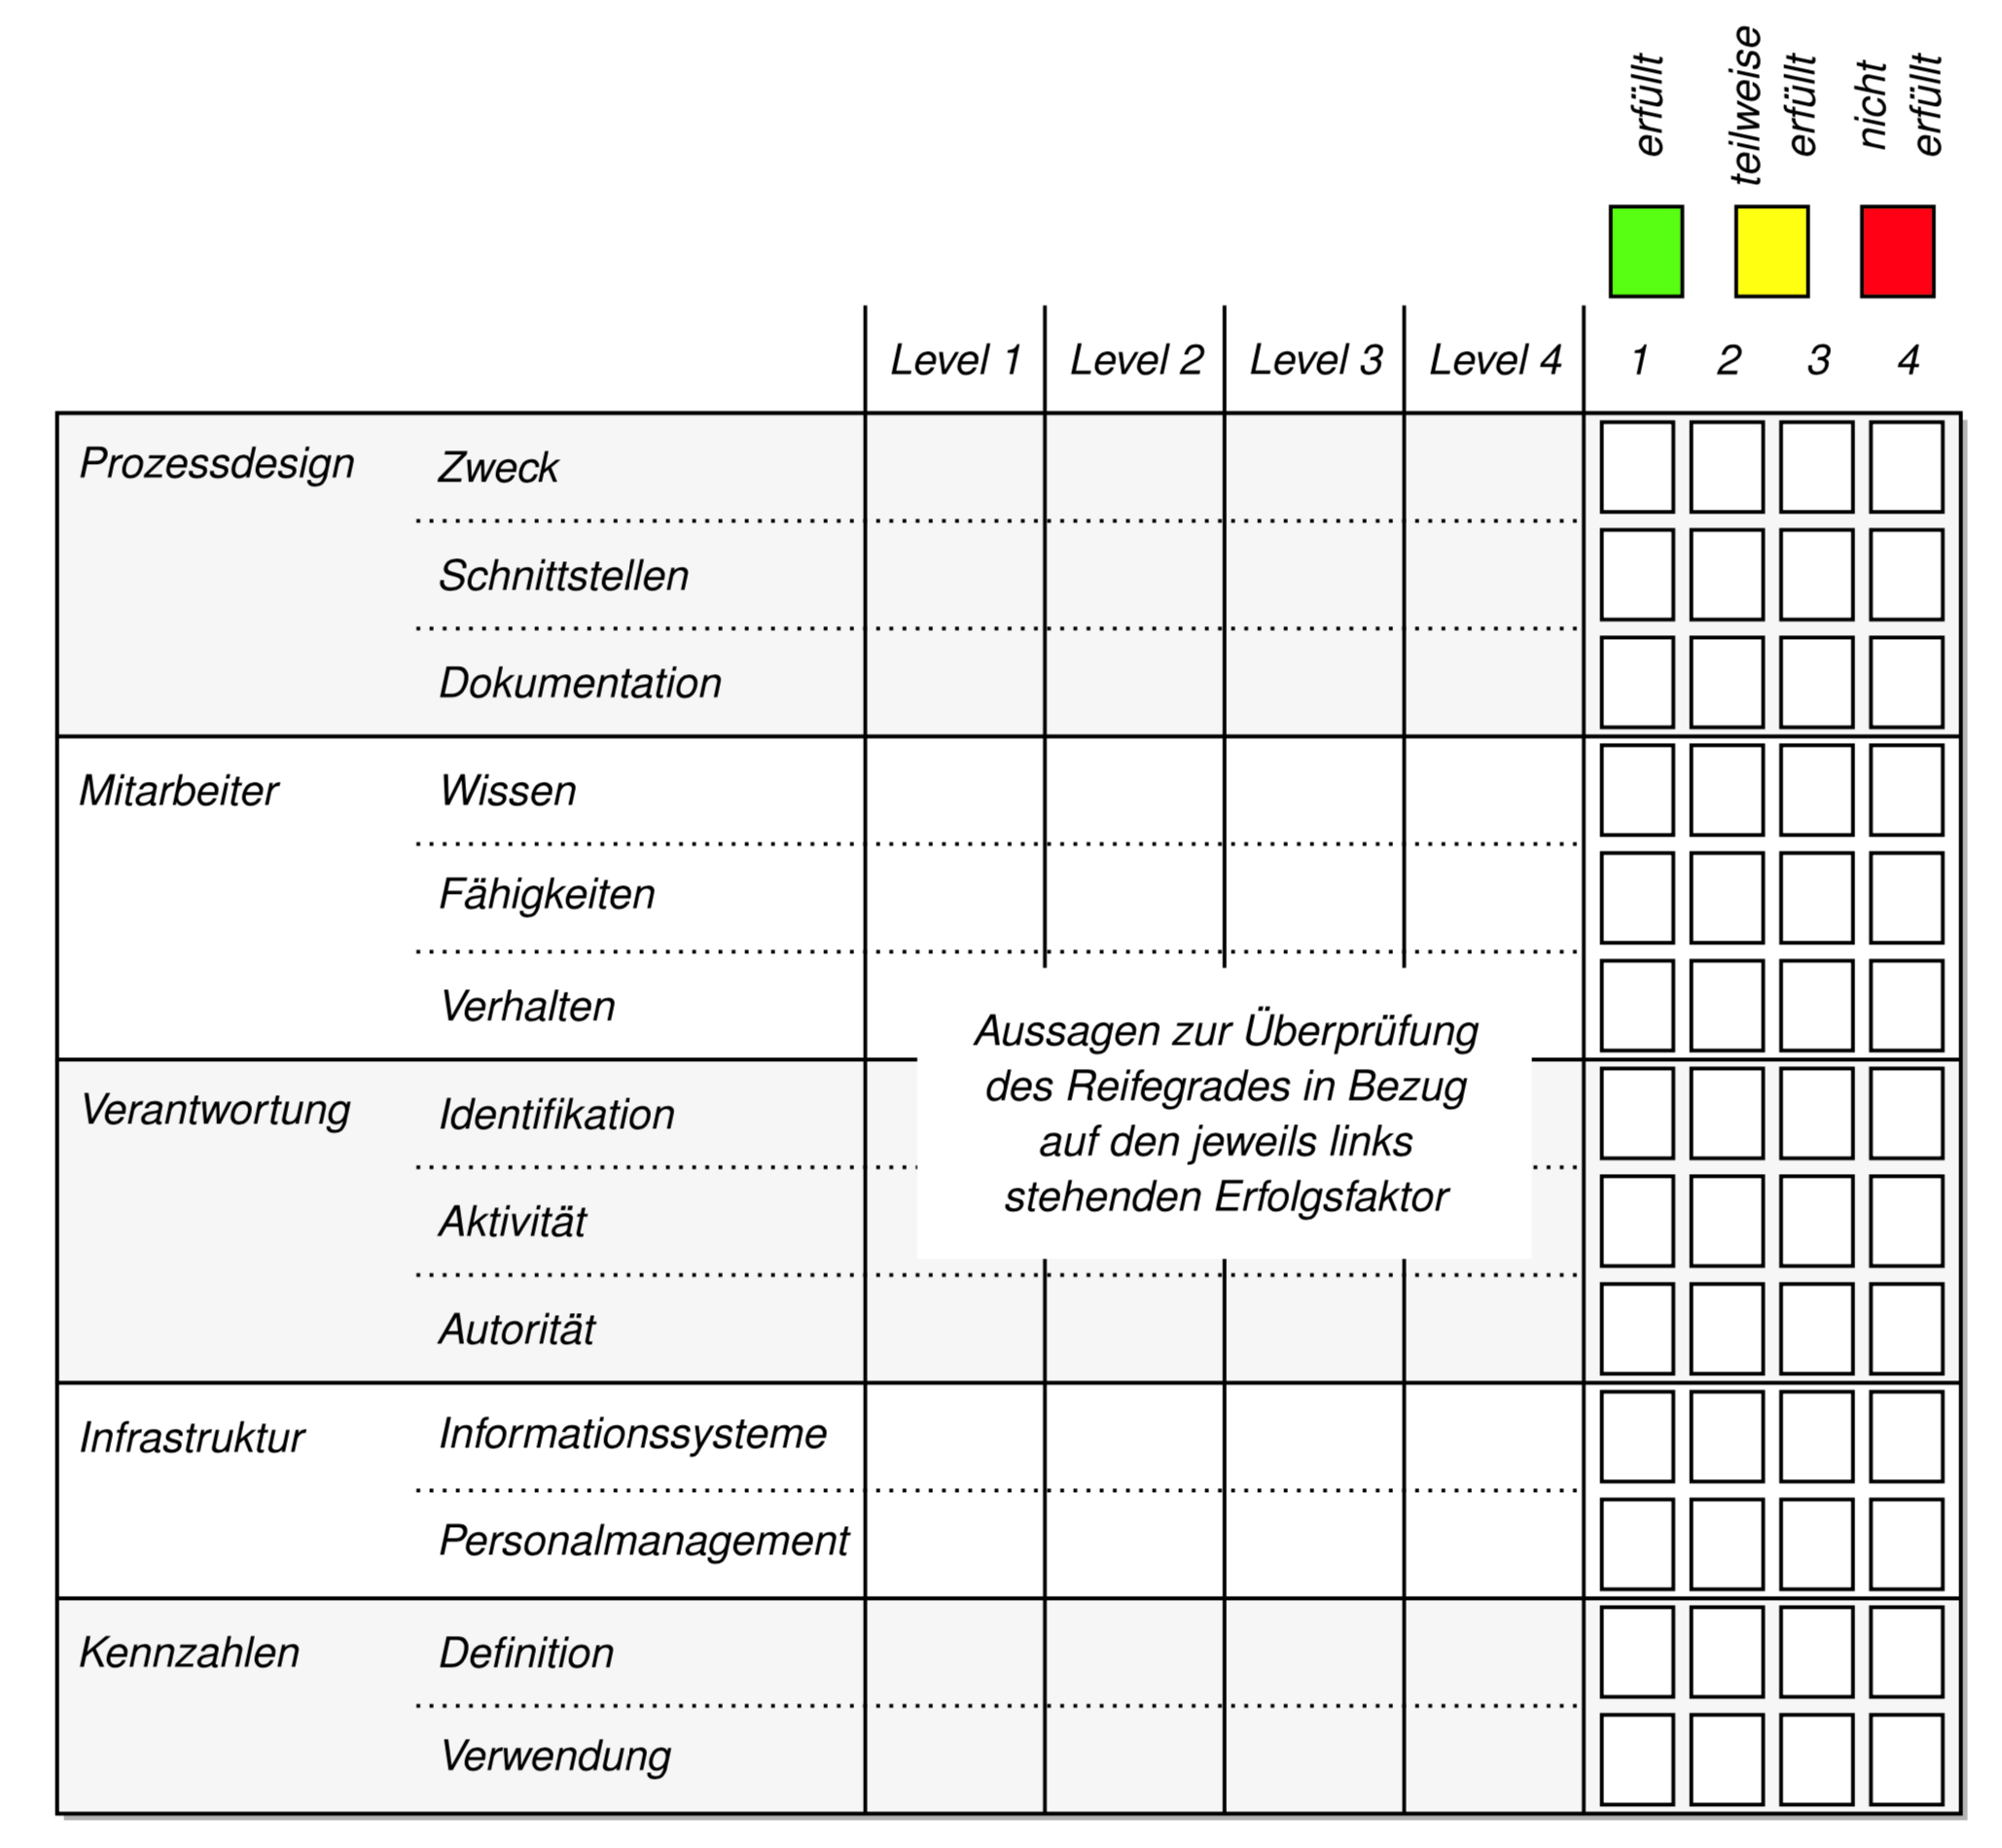
\includegraphics[width=12cm]{schemareifegradpemm.png}
  \caption*{\footnotesize{\textbf{Quelle:} \cite[S.83]{Carlo2014}}}
  \label{fig:schemareifegradpemm}
\end{figure}

Wie man in \autoref{fig:schemareifegradpemm} erkennen kann, sind die Prozessdeterminanten in Subbereiche aufgeteilt. Zum Beispiel wird die Prozessdeterminante Prozessdesign,in die Subbereiche Zweck, Schnittstellen und Dokumentation unterteilt. Durch verschiedene Aussagen werden diese in die Reifegradstufen P1 bis P4 bei den Prozessdeterminanten und E1 bis E4 bei den Unternehmenskompetenzen bewertet.\par
Die Reifegradstufen bauen aufeinander auf, weshalb die Anforderungen der darunterliegenden Stufen bereits erfüllt sein müssen bevor eine höhere Stufe erreicht werden kann. Wenn eine Aussage als weitgehend zutreffend gilt, also mindestens zu 80\% erfüllt ist, dann ist die entsprechende Reifegradstufe erreicht und das Kontrollfeld wird grün eingefärbt.\par
Ist die Aussage weitgehend falsch, also zu weniger als 20\% erfüllt, dann ist die entsprechende Reifegradstufe nicht erreicht und das Kontrollfeld wird rot eingefärbt. In allen anderen Fällen gilt die Reifegradstufe als teilweise erreicht und das Kontrollfeld wird gelb eingefärbt (vgl. \cite[S.83]{Carlo2014}). \par

Der zweite Fragebogen bzw. das Schema für die Unternehmensbewertung folgt demselben Prinzip. Nachfolgend sind die vier Unternehmenskompetenzen näher aufgeführt:

\begin{itemize}
  \item \textbf{Leadership} \par Inwieweit werden Prozessveränderungen durch das Topmanagement mitgetragen oder vorangetrieben?
	\item \textbf{Unternehmenskultur} \par Wie groß ist die Akzeptanz gegenüber Veränderungen innerhalb der Belegschaft? Und wie gut funktioniert das Teamwork?
	\item \textbf{Erfahrungen} \par Inwieweit verfügt das Unternehmen über Erfahrung mit der Neugestaltung von Prozessen?
	\item \textbf{Steuerung} \par Wie gut wird das Management von Veränderungen durch Systeme und Strukturen unterstützt?
\end{itemize}

(vgl. \cite[S.43]{Bensiek2013})

\autoref{fig:pemmunternehmenskom} zeigt einen Ausschnitt des beispielhaft ausgefüllten Fragebogens für die Unternehmenskompetenz Leadership mit allen zu bewertenden Aussagen.

\begin{figure}[H]
  \centering
  \caption{Bestimmung des Leistungstandes der Unternehmenskompetenzen nach \acs{pemm}}
  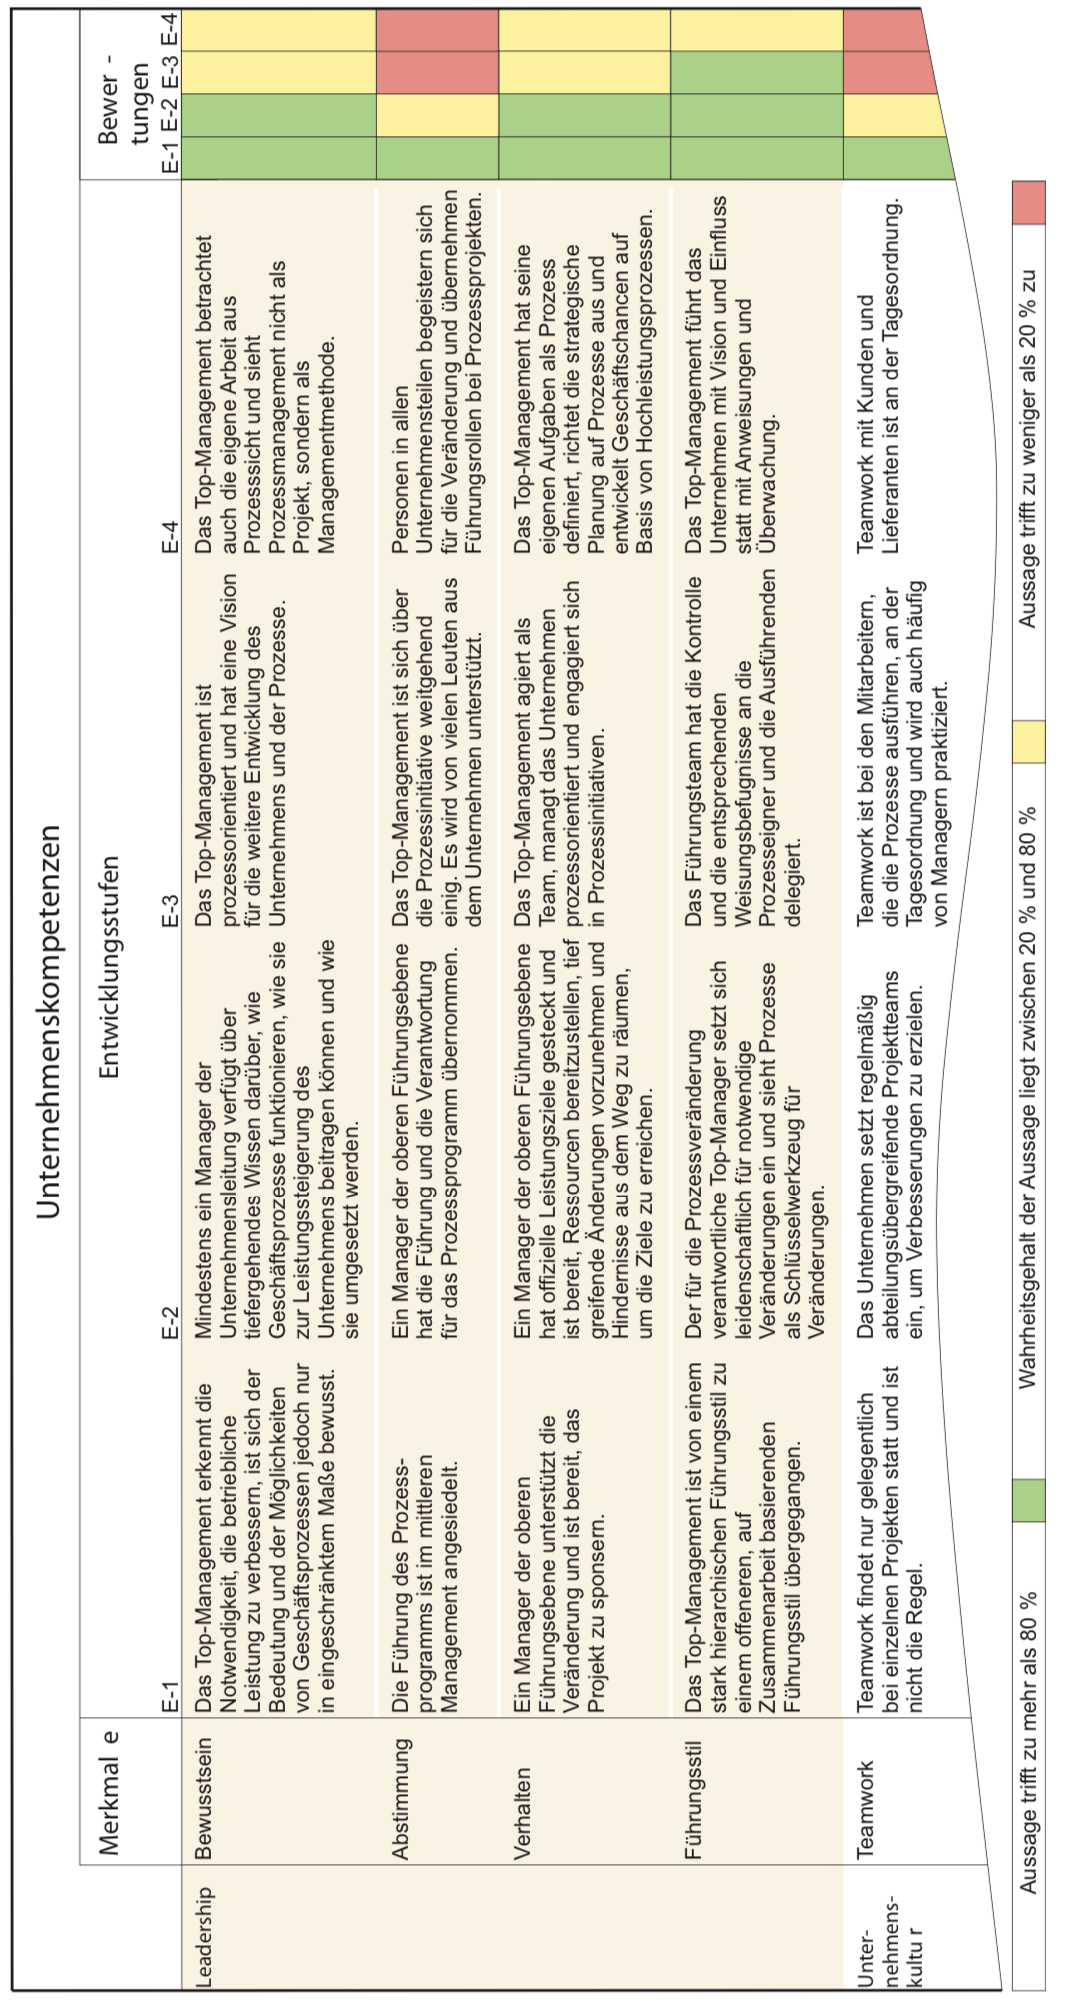
\includegraphics[width=12cm]{pemmunternehmenskom.png}
  \caption*{\footnotesize{\textbf{Quelle:} \cite[S.42]{Bensiek2013}}}
  \label{fig:pemmunternehmenskom}
\end{figure}

Nach der Bewertung aller Subbereiche können die Prozess- und Unternehmensreifegrade ermittelt werden. Da der Reifegrad einer Prozessdeterminante oder Unternehmenskompetenz nur so gut wie sein schwächster Subbereich ist, ist die Reifegradstufe der Prozessdeterminante bzw. der Unternehmenskompetenz gleich der Stufe des jeweils am niedrigsten bewerteten Subbereichs. Um Veränderungen zu erkennen und beispielsweise Fortschritte aufzuzeigen, kann der Reifegrad mit vorrangegangenen Erhebungen verglichen werden (vgl. \cite[S.43f]{Bensiek2013}).\par
Nach \acs{pemm} kann sich jedes Unternehmen durch das Erreichen von höheren Reifegradstufen verbessern. Es ist also erstrebenswert, den höchsten Reifegrad in diesem Modell zu erreichen bzw. Schwachstellen aufzudecken und ein homogenes Profil anzustreben. Schwachstellen werden durch niedriger ausgeprägte Subbereiche aufgezeigt und können so vom Unternehmen im Rahmen von Optimierungen fokussiert werden (vgl. \cite[S.44]{Bensiek2013}).\par
Es bietet sich an, das Modell von verschiedenen Hierarchieebenen des Unternehmens betrachten zu lassen, da üblicherweise die Einschätzungen des Managements wesentlich positiver ausfallen als die der Mitarbeiter. Ist dies der Fall, sollte man der Ursache der unterschiedlichen Einschätzung auf den Grund gehen. Die Fragebögen werden im Rahmen von Interviews, Diskussionsrunden oder Workshops besprochen und bewertet (vgl. \cite[S.43]{Bensiek2013}).

\subsubsection{Bewertung von \acs{pemm}}

PEMM ist ein einfaches und pragmatisches Reifegradmodell, das sich auf alle Unternehmen in jeglichen Branchen anwenden lässt. Das Unternehmen kann das Modell schnell und einfach selbst anwenden, da kein geschultes Personal oder externe Beratung erforderlich sind. \par Die Leistungsbewertung basiert auf Erfahrungen in der Praxis. Zudem sind die Fragebögen kostenlos erhältlich, weshalb dieses Modell eine kostengünstige Variante darstellt, um den Reifegrad eines Unternehmens zu bewerten und um Lücken im System aufzudecken. Die Ergebnisse der Analyse sind vergleichbar, allerdings wird keine Unterstützung für einen Vergleich von diesem Modell gegeben.\par Konkrete Empfehlungen für die Verbesserungen werden nicht genannt und müssen individuell erarbeitet werden. Ein weiterer Nachteil stellt die fehlende Softwareunterstützung für dieses Modell dar (vgl. \cite[S.44]{Bensiek2013}).

\subsection{SPICE}

\ac{spice} war ein Projekt aus dem die ISO/IEC 15504 Norm entstanden ist. Sie ist ein internationaler Standard, über den Prozesse bewertet werden können.
Die Entwicklung der Norm wurde durch die Softwareentwicklungsprozesse geprägt und später auch in Bereichen, wie Automotive verwendet.\par
Die Einstufung erfolgt auf sechs Stufen, die jeweils keine bis zwei Attribute besitzen. Dabei wird ein Bewertungsrahmen eingesetzt, um festzustellen, wie gut ein Prozess durchgeführt wird.\par
Im Standard werden auch Best Practice Beispiele bereitgestellt, an denen sich die Umsetzung orientieren kann.

\subsubsection{Reifegraddimensionen}

Die Einschätzung des Reifegrads der Prozesse findet dabei unter zwei Dimensionen statt. Es werden Prozesse ausgewählt, meistens aus einem Bereich (Einkauf, Verkauf, etc.) und dann in den Reifegrad eingestuft. Die Reifegrade bestehen dabei aus null bis zwei Attributen. In der nachfolgenden \autoref{fig:spicedimensionen} können die Attribute eingesehen werden.

\begin{figure}[H]
  \centering
  \caption{Reifegradstufen und Prozessattribute}
  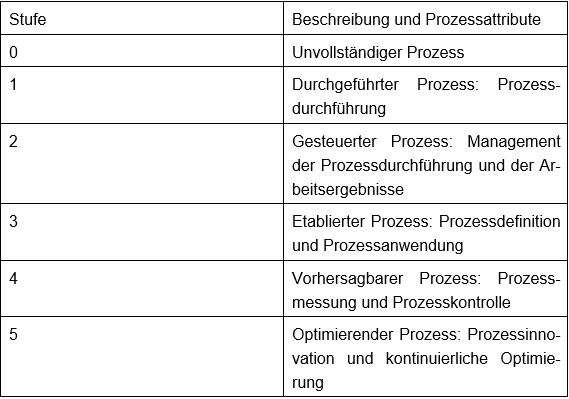
\includegraphics[width=12cm]{spicedimensionen.png}
  \label{fig:spicedimensionen}
\end{figure}

Die Prozesse des Unternehmens werden in drei Kategorien unterteilt:

\begin{itemize}
  \item \textbf{Primäre Prozesse} \par \glqq Die Kategorie primäre Prozesse im Lebenszyklus umfasst alle Prozesse, die vom Kunden genutzt werden können, wenn er Produkte von einem Lieferanten erwirbt. Dazu auch vom Lieferanten, wenn er darauf reagiert und Produkte an den Kunden liefert. Dazu zählen auch die für Spezifikation, Design, Entwicklung, Integration und Tests erforderlichen Engineering-Prozesse.\grqq{} \par
  Die primären Prozesse werden wiederum in die Gruppen Acquisition Prozessgruppe, Supply Prozessgruppe und Engineering Prozessgruppe unterteilt.\par
  Die Acquisition Prozessgruppe umfasst alle Prozesse, um ein Produkt oder Dienstleistung zu erwerben. Darunter fallen Vertragsvereinbarungen, Lieferanten Monitoring, Technische Anforderungen, rechtliche und administrative Anforderungen, Projektanforderungen, Ausschreibungen und Lieferanten-qualifizierungen.\par
  Die Supply Prozessgruppe umfasst alle Prozesse, um ein Produkt oder Dienstleistung zu erbringen. Darunter fallen Angebotsabgabe des Lieferanten und Produktfreigabe.\par
  Die Engineering Prozessgruppe umfasst alle Prozesse, um die Kundenanforderungen zu ermitteln und zu verwalten, das Produkt zu spezifizieren und zu implementieren. Diese Prozessgruppe ist stark an der Softwareentwicklung orientiert. Darunter fallen Anforderungserhebung, Systemanforderungsanalyse, Entwurf der Systemarchitektur, Softwareanforderungsanalyse, Entwurf des Softwaredesigns, Softwareerstellung, Softwareintegrationstest, Softwaretest, Systemintegrationstest und Systemtests.

	\item \textbf{Unterstützende Prozesse} \par Die unterstützenden Prozesse helfen anderen Prozessen an verschiedenen Punkten des Lebenszyklus. Dazu gehören Qualitätssicherung, Verifikation, Gemeinsames Review, Dokumentation, Konfigurationsmanagement, Problemlösungsmanagement und Änderungsmanagement.
	\item \textbf{Organisatorische Prozesse} \par Die Kategorie der organisatorischen Prozesse umfasst alle Prozesse, die zur Zielerreichung der Organisation dienen. Diese werden in die Gruppen Management Prozessgruppe, Prozessverbesserungs Prozessgruppe und Reuse Prozessgruppe unterteilt.
  Die Management-Prozessgruppe umfasst alle Prozesse, die ein beliebiges Projekt oder einen beliebigen Prozess leiten. Darunter fallen Projektmanagement, Risikomanagement und Messung.\par
  Die Prozessverbesserungs Prozessgruppe umfasst alle Prozesse, die zur Definition, Anwendung und Verbesserung von Prozessen durchgeführt werden. Darunter fällt die Prozessverbesserung.\par
  Die Reuse Prozessgruppe umfasst alle Prozesse, die zur systematischen Nutzung von Reuse-Programmen beitragen. Darunter fällt das Reuse Programm Management.

\end{itemize}

Das gesamte Konzept wird in \autoref{fig:spicedimensionen2} nochmals genauer dargestellt.

\begin{figure}[H]
  \centering
  \caption{Reifegraddimensionen}
  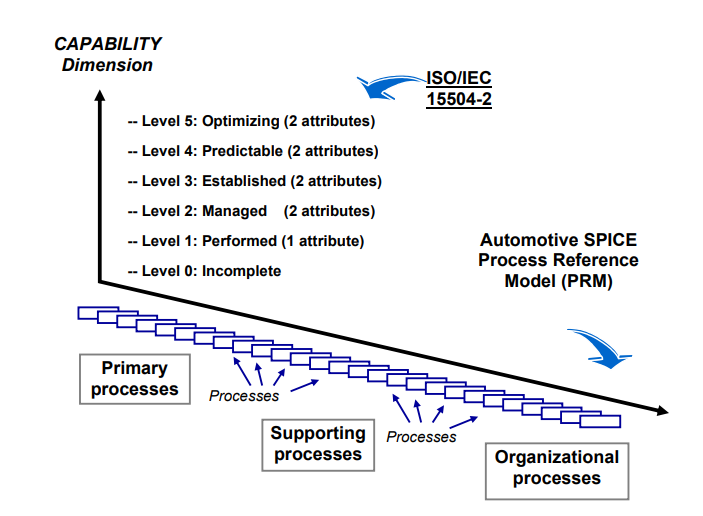
\includegraphics[width=12cm]{spicedimensione2.png}
  \label{fig:spicedimensionen2}
\end{figure}


\subsubsection{Indikatoren für die Prozessfähigkeit}

Um den Erfolg der Verbesserung einer Prozessfähigkeit zu messen, müssen zwei generische Indikatoren definiert werden. Zum einen Generic Practises, welche die groben Aktivitäten des Prozesses definiert und dazu als Hilfe-stellung zur Implementierung der Attribut-Charakteristika dient. Zum anderen werden Gerneric Ressources definiert, welche die Ressourcen, die zur Zielerreichung benötigt werden, definieren. Darunter fallen Personal, Werkzeuge und Hilfsmittel, sowie Methoden und Infrastruktur.

\subsubsection{Indikatoren für die Prozessdurchführung}

Um den Erfolg der Verbesserung einer Prozessdurchführung zu messen, müssen zwei Indikatoren definiert werden. Zum einen müssen Base Practises definiert werden, welche die einzelnen Aktivitäten zur Erfüllung des Prozesszwecks darstellen. Zum anderen müssen Work Products definiert werden, welche die Ausgabeobjekte beziehungsweise die Eingabeobjekte für den nächsten Prozess darstellen.

\subsubsection{Durchführung}

In der ISO/IEC 15504 wird außerdem genau beschrieben, wie die Durchführung eines Assessments aussehen und dokumentiert werden muss. Die folgenden Aktivitäten müssen mindestens enthalten sein:

\begin{itemize}
  \item \textbf{Planung}
	\item \textbf{Datensammlung}
	\item \textbf{Datenvalidierung}
	\item \textbf{Bewertung der Prozessattribute}
	\item \textbf{Berichtswesen}
\end{itemize}

In den Eingaben für das Assessment werden Zweck und Umfang bestimmt, also welche Prozesse bis zu welchem Fähigkeitsgrad untersucht werden sollen. In der Ausgabe wird das Ergebnis präsentiert.

Eine typische Durchführung kann in folgenden Schritten durchgeführt werden:

\begin{itemize}
  \item 1. Ein Steuerungsteam bilden
	\item 2. Ziele für die Umsetzung setzen
	\item 3. Die für die Durchführung relevanten Prozesse identifizieren
	\item 4. Prozessteams bilden
	\item 5. Ressourcen und Zeit für die Durchführung schaffen
	\item 6. Die Reifegrade der relevanten Prozesse feststellen
	\item 7. Einen Verbesserungsplan für die einzelnen Prozesse erstellen
	\item 8. In regelmäßigen Abständen den Status der Verbesserung beobachten
	\item 9. Die Steuerungsgruppe regelmäßig über den Status informieren
	\item 10. Zusätzliche Ressourcen bereitstellen, falls welche benötigt werden
	\item 11. Den Reifegrad der Prozesse erneut messen
	\item 12. Neue Ziele für die Umsetzung setzen
\end{itemize}

\subsubsection{Vorteile}

Die Vorteile von \acs{spice} sind unter anderem:

\begin{itemize}
  \item Anerkannter Nachweis für Ihre Entwicklungskompetenz
	\item Gute Sichtbarkeit der Stärken und Schwächen Ihrer Entwicklungsprozesse
	\item Fortlaufende Verbesserung abgestimmter und eindeutig festgelegter Prozesse
	\item Gezielte Berücksichtigung der Best Practices im Assessmentmodell
	\item Deutliche Reduzierung von Risiken und Fehlleistungskosten
	\item Bei Lieferantenassessments ist der Prozessreifegrad für die Kunden erkennbar
\end{itemize}

\subsection{Business Process Maturity Model}

Das \ac{bpmm} ist ein Reifegradmodell, dass durch das herstellerunabhängige Industriekonsortium \ac{omg} entwickelt worden ist.
Die 1989 gegründete OMG umfasst über 800 Mitglieder von Unternehmen, wie z.B. Microsoft, Apple und IBM, die sich um die Entwicklung von Standards in der IT-Branche befassen.\par
Bekannte internationale Standards sind zum Beispiel die Unified Modeling Language zur Modellierung und Dokumentation von objektorientierten Systemen
und die grafische Geschäftsprozessmodellierung mit Business Process Modeling Notation. Der Reifegrad wird in fünf Stufen unterteilt, die in der 482 Seiten langen Veröffentlichung von OMG detailliert beschrieben werden.

\subsubsection{Reifegradstufen im \acs{bpmm}}

\begin{figure}[H]
  \centering
  \caption{\acs{bpmm}-Reifegradstufen}
  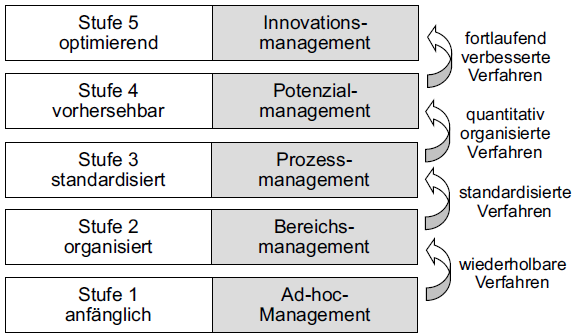
\includegraphics[width=12cm]{bpmmreifegradstufen.png}
  %\caption*{\footnotesize{\textbf{Quelle:} \cite[,2019,o.S.]{Capgemini2019}}}
  \label{fig:reifegradstufen}
\end{figure}

Bei \acs{bpmm} werden die Reifegrade in fünf Stufen unterteilt, siehe \autoref{fig:reifegradstufen}. Die \acs{omg} spricht hierbei von „maturity levels“ die aufeinander aufbauen. Ist eine Stufe erreicht, so gelten die vorherigen Voraussetzungen zum Erreichen dieser Reifegradstufe auch als erfüllt.
\textbf{Reifegradstufe 1 (initial)} ist ein Unternehmen, bei denen die Prozesse unvorhersehbar ablaufen. Die Unternehmensführung betreibt Ad-hoc-Management, bei dem nur bei konkret vorliegenden Problemen in Prozesse eingegriffen wird. Die Prozessqualität wird maßgeblich durch die Kompetenz der Mitarbeiter bestimmt. Maßnahmen zu einer kontinuierlichen Prozessverbesserung fehlen vollständig.
\par
\textbf{Reifegradstufe 2 (managed)} trifft zu, wenn auf Bereichs- beziehungsweise Abteilungsebene eine Management-Funktion zur Stabilisierung der Prozesse vorhanden ist. Die gelten jedoch nur für einen Bereich. Die Zusammenlegung von Bereichsübergreifenden (ähnlichen) Prozessen findet noch nicht statt und kann zu unterschiedlich angewendeten Verfahren für ähnliche Prozesse führen. Die Mitarbeiter arbeiten bereits mit wiederholbaren Prozessen, die lokal und operativ überwacht werden.
\par
\textbf{Reifegradstufe 3 (standardized)} besitzt erstmals Bereichsübergreifende Prozesse. Die Geschäftsprozesse sind standardisiert und erleichtern die Produkterstellung. Prozessverbesserungen werden bereits vorgenommen. Ein Prozessmanagement hält schriftlich erstmals bestimmte Verfahrensregeln fest und definiert Qualitätskriterien, die sich mit betriebswirtschaftlichen Kennzahlen messen lassen. Diese Kennzahlen und Kriterien sind eine erste Maßnahme zur Verbesserung einer Gesamtunternehmensplanung.
\par
\textbf{Reifegradstufe 4 (predictable)} setzt auf statistische Verfahren zur Messung von Prozessqualität. Die Ergebnisse aus Prozessen werden damit nicht nur planbar, sondern auch vorhersehbar. Ein Potenzialmanagement bewertet und überwacht die Arbeitsabläufe, um Verfahrensvarianten erkennen, verstehen und kontrollieren zu können. Erfahrungen aus der Anwendung von Standardprozessen werden mit den Arbeitseinheiten geteilt, damit weitere Prozessoptimierungen vorgenommen werden.
\par
\textbf{Reifegradstufe 5 (innovating)} bezeichnet eine Organisation, dessen interne Geschäftsprozesse optimiert sind und kontinuierlich verbessert werden. Ein Innovationsmanagement sorgt organisationsübergreifend für systematische Prozessverbesserungen, die durch ein Change Management umgesetzt werden.
\par

Details zu den einzelnen Stunfen können in nachfolgender \autoref{fig:bpmmreifegrade} angesehen werden.

\begin{figure}[H]
  \centering
  \caption{Details der Reifegradstufen im \acs{bpmm}}
  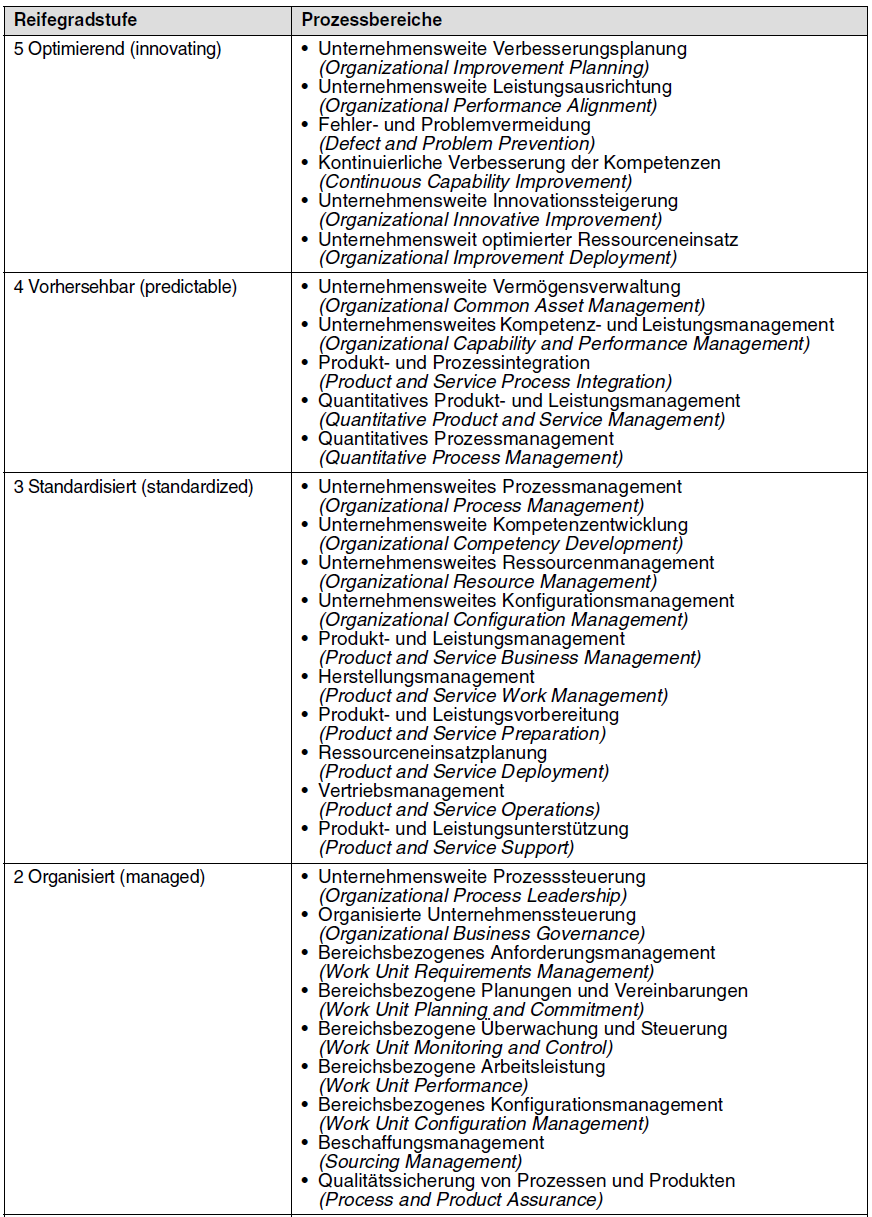
\includegraphics[width=12cm]{bpmmreifegrade.png}
  %\caption*{\footnotesize{\textbf{Quelle:} \cite[,2019,o.S.]{Capgemini2019}}}
  \label{fig:bpmmreifegrade}
\end{figure}

\subsubsection{Prozessbereiche und Zielesystematik}

Zur Ermittlung ob ein Reifegrad erreicht wurde müssen die Anforderungen der Prozessbereiche erfüllt werden. Jeder Reifegrad besteht aus fünf bis zehn Prozessbereichen. Jeder Prozessbereich wird wiederum in Ziele und Teilaktivitäten gegliedert. Die Teilaktivitäten sind die konkreten Anforderungsbeschreibungen, ohne explizit eine anzuwendende Methode anzugeben. Dadurch können Prozessbereiche auch durch bereits vorhandene Methoden erfüllt sein.

\subsubsection{Verantwortlichkeiten}

Damit die definierten Ziele der Prozessbereiche umgesetzt werden, werden diese bestimmten Unternehmensbereichen zugeteilt. \acs{bpmm} unterscheidet in die vier Unternehmensbereiche „Unternehmensleitung“, „mittleres Management“, „Querschnittsbereiche“ und „Ausführungsebene“. Eine Übersicht dieser Zuteilung und die jeweilige Reifegradstufe pro Prozessbereich sind in der nachfolgenden \autoref{fig:verantwortlichkeiten} ersichtlich.

\begin{figure}[H]
  \centering
  \caption{\acs{bpmm} Verantwortlichkeiten}
  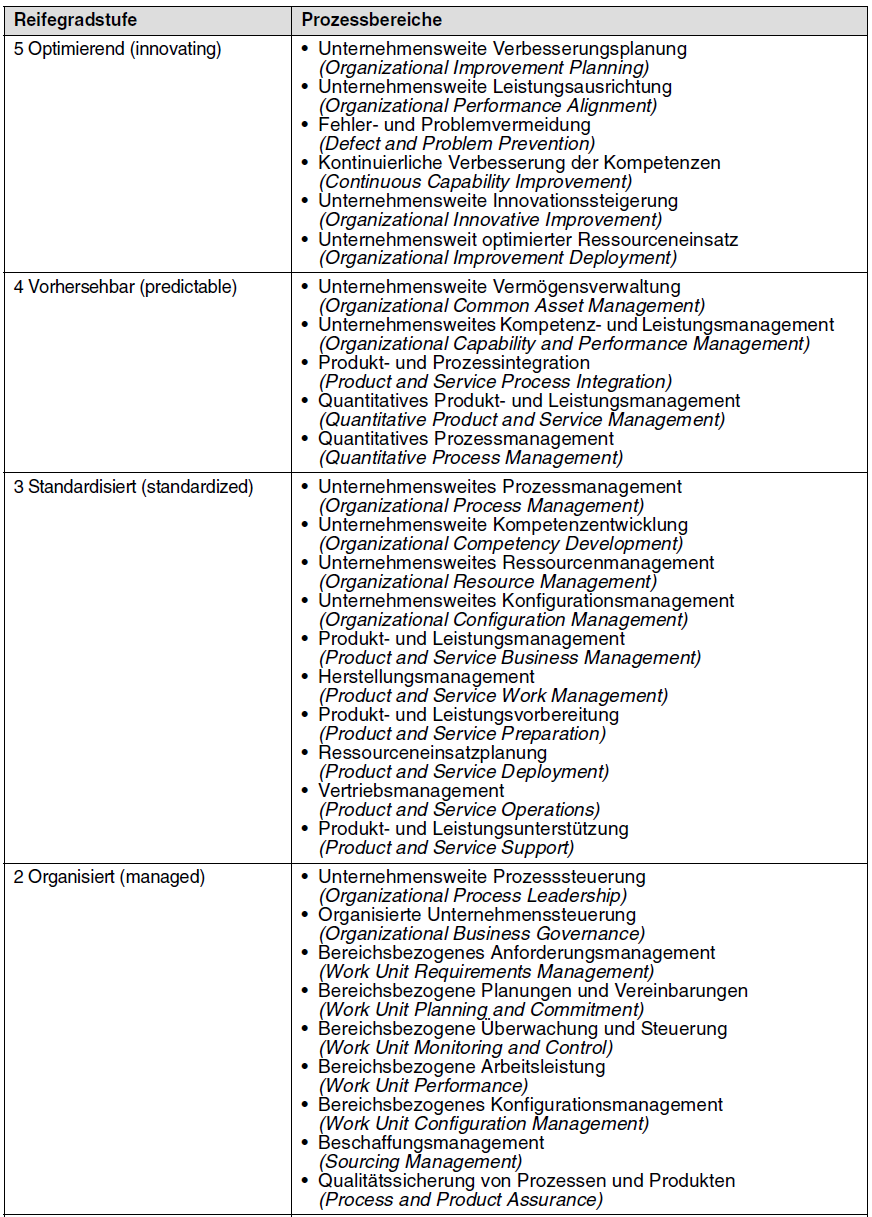
\includegraphics[width=12cm]{bpmmreifegrade.png}
  %\caption*{\footnotesize{\textbf{Quelle:} \cite[,2019,o.S.]{Capgemini2019}}}
  \label{fig:verantwortlichkeiten}
\end{figure}

Die Unternehmensleitung übernimmt dabei die unternehmensweiten Prozess- und Produktmanagement Aufgaben. Wichtige Ziele sind die kontinuierliche Verbesserung von Prozessen und der optimale Ressourceneinsatz. \par
Das mittlere Management kümmert sich um das bereichsbezogene Aufgabenmanagement. Dabei werden innerhalb der durch die Unternehmensleitung vorgegeben Handlungsrahmen quantitative Ziele umgesetzt. Auch die Überwachung und Steuerung des Bereichs fallen zu den Verantwortlichkeiten des mittleren Managements.\par
Die Querschnittsbereiche (Steuerungs- und Revisionseinheiten) unterstützen die Maßnahmen durch die exakte Dokumentation bestehender Prozesse, um daraus Verbesserungspotenziale ableiten zu können. Es werden Stärken und Schwächen der Prozesse identifiziert. \par
Die Ausführungsebene besteht aus den Arbeitseinheiten und damit der unmittelbaren Wertschöpfungsquelle. Hier werden die Prozessverbesserungen operativ umgesetzt und quantitatives Prozessmanagement betrieben.

\subsubsection{Einsatzmöglichkeiten}

Das \acs{bpmm} lässt sich grundsätzlich in allen Branchen nutzen. Der Einsatz erfolgt durch konkrete und individuell festgelegte Methoden des Unternehmens, da \acs{bpmm} nur detaillierte Anforderungen und keine Methoden vorgibt.\par
Problematisch sehen Hogrebe und Nüttgens die eindeutige Zuordnung von Prozessbereichen zu Verantwortungsebenen, bei denen keine Verantwortlichkeiten zu unternehmensübergreifenden Prozessen im \acs{bpmm} definiert sind. Ein weiterer Punkt ist der Fokus auf ausschließliche Optimierung der Geschäftsprozesse ohne Angleichung der Aufbau- und Ablauforganisation.\par
Mit \acs{bpmm} werden die detailliert formulierten Anforderungen im Unternehmen dauerhaft verankert und erzeugt eine Unternehmenskultur, die eine stetige Prozessverbesserung in allen Bereichen anstrebt. \acs{bpmm} bietet alternativ auch die Möglichkeit, nur teilweise in bestimmten Bereichen angewendet zu werden.\par
Abschließend nennen Hogrebe und Nüttgens das \acs{bpmm} ein klar strukturiertes Reifegradmodell mit einer hohen Detailtiefe bei der Beschreibung erforderlicher Schritte zur Erreichung von Reifegradstufen. Der Einsatz von \acs{bpmm} sollte jedoch von der Geschäftsleitung wohlüberlegt sein, da dies zu einem Eingriff in die Organisationsstruktur führt und Ressourcen bindet.
